\documentclass[12pt,a4paper,openright,twoside]{book}
\usepackage[utf8]{inputenc}
\usepackage{disi-thesis}
\usepackage{code-lstlistings}
\usepackage{notes}
\usepackage{shortcuts}
\usepackage{acronym}

\setlength{\parindent}{0pt}
\setlength{\parskip}{6pt}

\school{\unibo}
\programme{Corso di Laurea Magistrale in Digital Transformation Management}
\title{Fancy Title}
\author{Andrea Giovanardi}
\date{\today}
\subject{Business Intelligence}
\supervisor{Matteo Golfarelli}
\cosupervisor{Dott. CoSupervisor 1}
\morecosupervisor{Dott. CoSupervisor 2}
\session{II}
\academicyear{2025-2026}

% Definition of acronyms
\acrodef{AI}{Artificial Intelligence}
\acrodef{BI}{Business Intelligence}
\acrodef{LLM}{Large Language Model}
\acrodef{RAG}{Retrieval-Augmented Generation}
\acrodef{OLAP}{Online Analytical Processing}
\acrodef{KPI}{Key Performance Indicator}
\acrodef{DS}{Delivery Station}

\mainlinespacing{1.241} % line spacing in mainmatter, comment to default (1)

\begin{document}

\frontmatter\frontispiece

\begin{abstract}    
Max 2000 characters, strict.
\end{abstract}

\begin{dedication} % this is optional
Optional. Max a few lines.
\end{dedication}

%----------------------------------------------------------------------------------------
\tableofcontents   
\listoffigures     % (optional) comment if empty
\lstlistoflistings % (optional) comment if empty
%----------------------------------------------------------------------------------------

\mainmatter

%----------------------------------------------------------------------------------------
\chapter{Introduction to the Problem}
\label{chap:introduction}
%----------------------------------------------------------------------------------------

\section{Context}
During one of the audited weeks of my internship, the operational dashboard flagged a clear productivity gap at the station. 
The AI summary built on top of it explained the gap with full confidence, but the explanation produced was factually incorrect. 
It pointed to a structural metric that had little to do with the real cause of the difference, and proposed corrective actions and "why" analyses that no manager could realistically carry out.
I noticed the error , that morning, because i was familiar with the station and the metric, but a manager that reads the same paragraph on a busy day or even if less experienced could have easily take that for true and acted on it. 

That episode marked my thesis begin and frames the general problem it adresses: what happen when a \ac{LLM} is placed on top of a \ac{BI} dashboard and asked to turn numbers into decisons? 
That's a key question expecially considering the setting of a \ac{DS}. 
It's the final node of the logistick network, the place where package are sorted in the early morning and loaded onto routes to be delivered to final customers.
The station where i worked, DFV2 in Udine, runs on a standard daily rhythm: plan the day, run it, measure what happened, adjust for tomorrow. 
Manager controls the rhythm trought a large set of indicators that read every day to determine if any correction is needed. Normally the window to act is narrow so is important that a Manager doesn't get the picture late or even wrong otherwise the chances to fix it would be lost.

Among all the indicators that we used at the station

\section{Criticalities}
This highlighted a strict necessity for numerical fidelity and domain constraints, which are essential for reliable, on-the-field decision-making in a fast-paced logistics environment.

\section{Framework}
The primary research question and the supporting sub-questions that guide the entire thesis aim to address how an AI-BI data binding framework can be designed to guarantee such fidelity.

\paragraph{Structure of the Thesis}
The remainder of this document is organized as follows:

\begin{itemize}
    \item \textbf{Chapter 2} reviews the state of the art and related works, exploring current paradigms for data integration, evaluating hallucination metrics, and identifying the specific research gap in operational BI.
    
    \item \textbf{Chapter 3} introduces the case study, detailing the operational setting, the core metric, the pre-AI baseline, and the single-case methodology adopted during the internship.
    
    \item \textbf{Chapter 4} presents the proposed solution, detailing the conceptual innovation of the three-contract framework (tile-as-source, curated knowledge tree, and sanitizer) and the system architecture.
    
    \item \textbf{Chapter 5} focuses on the results and evaluation, analyzing the catalog of grounding failures and providing both quantitative controlled assessments and real-world qualitative evidence.
    
    \item \textbf{Chapter 6} discusses the findings, highlighting the thesis contributions and generalizability, acknowledging limitations, and outlining future research directions.
\end{itemize}
%----------------------------------------------------------------------------------------
\chapter{State of the Art and Related Works}
\label{chap:state_of_the_art}
%----------------------------------------------------------------------------------------

\section{Data Integration}
Main approaches for connecting LLMs to data, including Retrieval-Augmented Generation (RAG), prompt-based methods, tool use, and domain knowledge injection via semantic layers.

\section{Evaluation}
Existing metrics used to measure and evaluate AI hallucinations.

\section{Literature}
Current research and advancements in GenBI and LLM OLAP.

\section{Research Gap}
Identification of the specific gap in the current literature that this thesis aims to bridge by proposing a unified framework.

I suggest referencing stuff as follows: \cref{fig:random-image} or \Cref{fig:random-image}

\begin{figure}[h]
    \centering
    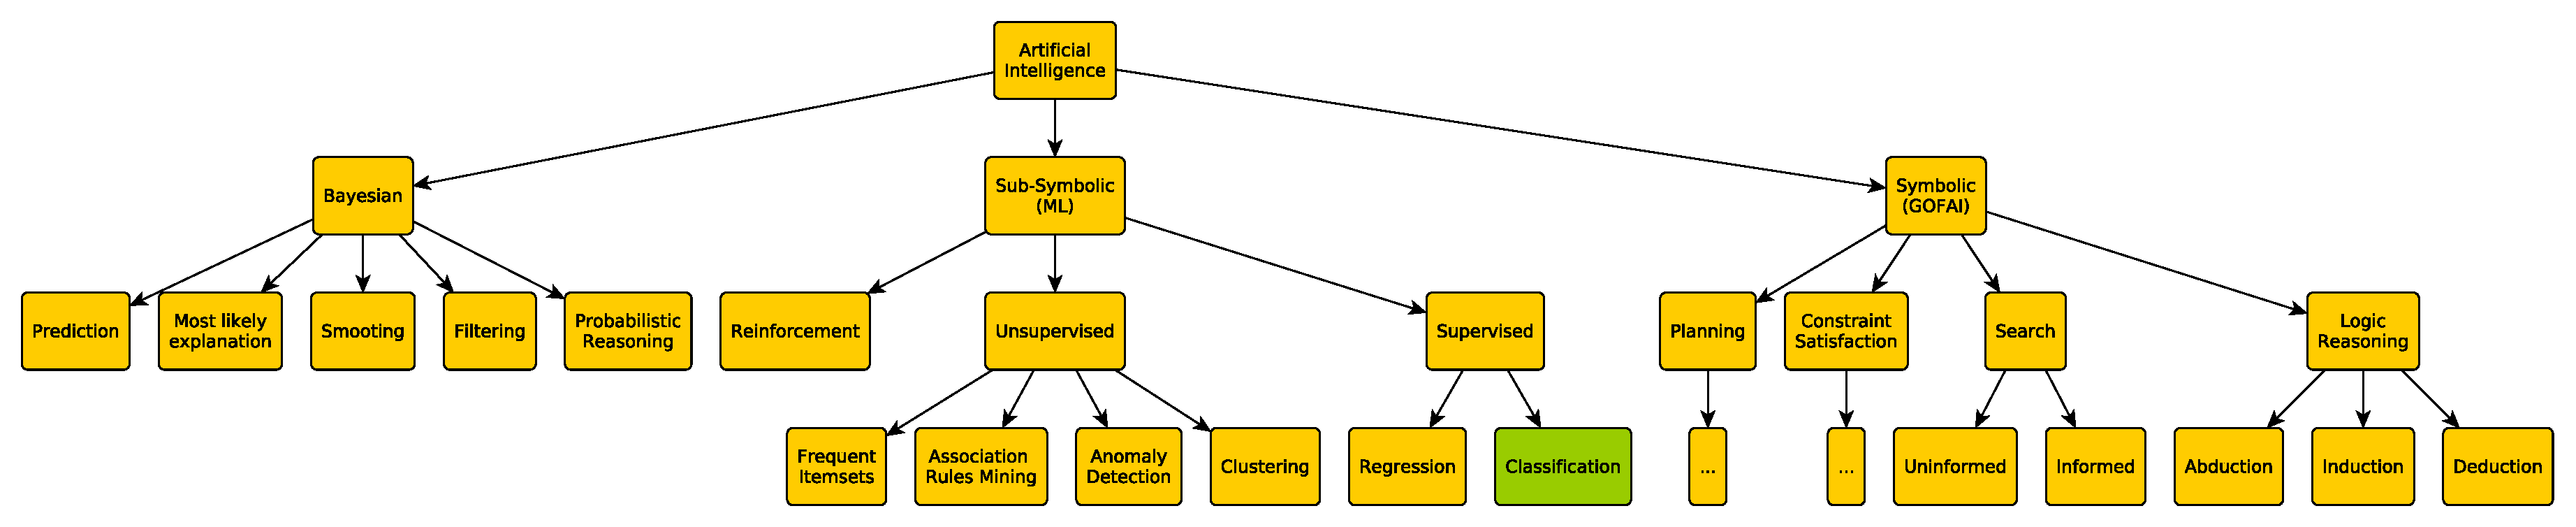
\includegraphics[width=.8\linewidth]{figures/random-image.pdf}
    \caption{Some random image}
    \label{fig:random-image}
\end{figure}

%----------------------------------------------------------------------------------------
\chapter{Case Study: Context and Problem}
\label{chap:case_study}
%----------------------------------------------------------------------------------------

\section{Setting}
The last-mile delivery station environment, the continuous improvement cycle (plan, execute, measure, adjust), and the time pressure that makes delayed data visibility a missed intervention window.

\section{Core Metric}
Definition of the reference indicator as a productivity ratio (output units divided by input resource), the gap between planned and actual values, and its additive decomposition into a fixed set of mutually-exclusive categories with a two-level hierarchy, heterogeneous aggregation weights, and a residual term that guarantees completeness.

\section{Pre-AI Baseline}
The manual workflow for monitoring (weekly cadence, tile-by-tile extraction) and for producing the bridge document (subjective cause selection, unconstrained ranking, experience-dependent actions).

\section{Three Weaknesses}
Limited reactivity, subjective root-cause selection, and analyst dependence, mapped explicitly to the three contracts proposed in Chapter 4.

\section{Methodology}
Single-case longitudinal design where the researcher is embedded in the operational team for six months. Development followed an iterative pattern: observe a failure in the AI output, isolate it, fix it, validate against real data, check for regressions. Failure instances were collected and classified into families for the analysis in Chapter 5. A synthetic dataset preserving the structural properties of the real data built for the controlled evaluation.

%----------------------------------------------------------------------------------------
\chapter{Proposed Solution: Three-Contract Framework}
\label{chap:proposed_solution}
%----------------------------------------------------------------------------------------

\section{Core Concept}
Introduction of the three contracts (tile-as-source, curated knowledge tree, and post-generation sanitizer) as a unified solution to the grounding problem, each acting at a different point of the generation chain.

\section{Prompt Engineering}
The design of the system prompt as an explicit encoding of fidelity rules, with one directive per observed failure mode rather than generic accuracy instructions.

\section{Architecture}
The overall system architecture of the AI-BI pipeline, from data aggregation to final narrative output.

\section{Application}
How the framework was derived from the iterative development of the case study, showing the concrete implementation of each contract.

You may also put some code snippet (which is NOT float by default), eg: \cref{lst:random-code}.

\lstinputlisting[float,language=Java,label={lst:random-code}]{listings/HelloWorld.java}

\section{Fancy formulas here} % Mantenuto dal template originale

%----------------------------------------------------------------------------------------
\chapter{Results and Evaluation}
\label{chap:results}
%----------------------------------------------------------------------------------------

\section{Failure Analysis}
A catalog of the main grounding failure modes observed and an explanation of how the proposed framework mitigates them.

\section{Quantitative Assessment}
A controlled evaluation using mock data to compare different system configurations.

\section{Qualitative Assessment}
Two to three real-world qualitative episodes drawn from the case study to provide practical, operational evidence of success.

%----------------------------------------------------------------------------------------
\chapter{Discussion and Future Directions}
\label{chap:discussion}
%----------------------------------------------------------------------------------------

\section{Synthesis}
How the observed results successfully answer the initial research question.

\section{Contributions}
The specific value added to the existing literature regarding LLMs and BI.

\section{Generalizability}
An assessment of how well the three-contract framework can be adapted and applied to other contexts or industries.

\section{Limitations}
A transparent look at the limits of the current thesis work.

\section{Future Developments}
Potential next steps, such as extending the framework to support interactive Q\&A functionalities based on the same underlying schema.

%----------------------------------------------------------------------------------------
% BIBLIOGRAPHY
%----------------------------------------------------------------------------------------

\backmatter

\nocite{*} % Remove this as soon as you have the first citation

\bibliographystyle{alpha}
\bibliography{bibliography}

\begin{acknowledgements} % this is optional
Optional. Max 1 page.
\end{acknowledgements}

\end{document}